\subsubsection{RS485}

El RS485 es un estándar de comunicación serial que se utiliza ampliamente en aplicaciones industriales y de automatización debido a su robustez y fiabilidad \cite{rs485}. A diferencia de otros protocolos de comunicación como UART o SPI, el RS485 permite la comunicación de múltiples dispositivos en un mismo bus de datos sin necesidad de agregar una línea de selección por cada dispositivo, lo que lo hace ideal para redes en las que se requiere que varios dispositivos compartan una única línea de comunicación. En la figura \ref{fig:res485} se visualiza un bus de RS485 con varios dispositivos conectados en modo \textit{half-duplex} (los dispositivos pueden enviar o recibir, pero no ambas cosas al mismo tiempo). \\ 

\begin{figure}[H]
    \centering
    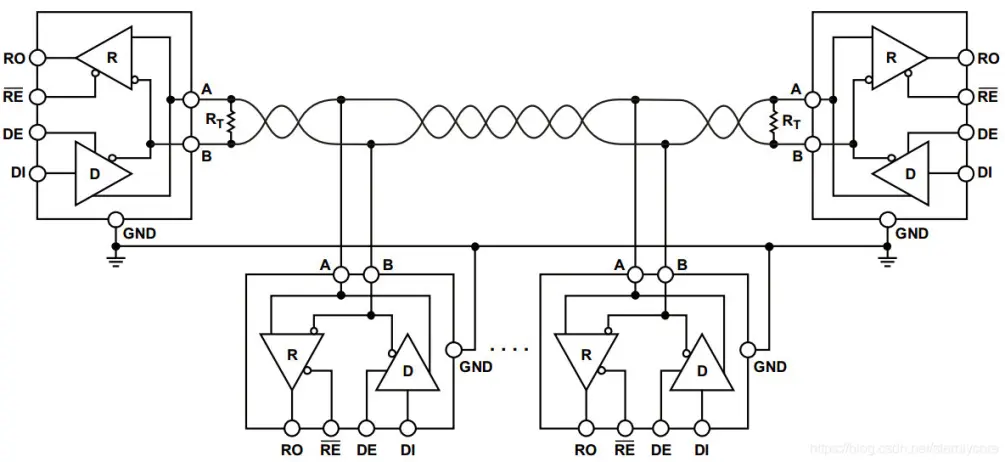
\includegraphics[width =  \linewidth]{img/rs485.png}
    \caption{Bus RS485 en modo \textit{half-duplex}}
    \label{fig:res485}
\end{figure}

Alguna de las características principales del protocolo RS485 son las siguientes: 

\begin{itemize}
    \item \textbf{Comunicación diferencial}: RS485 utiliza dos líneas para la transmisión de datos (A y B), lo que le permite operar bajo el principio de comunicación diferencial. Esto significa que el valor lógico de los datos se determina por la diferencia de tensión entre las dos líneas, lo que mejora la inmunidad al ruido y permite transmitir datos a largas distancias sin degradación de la señal.

    \item \textbf{Distancia y velocidad}: Puede transmitir datos a distancias de hasta 1200 metros, dependiendo de la velocidad de comunicación. A velocidades bajas (por ejemplo, 100 kbps), puede cubrir distancias más largas, mientras que a velocidades más altas (por ejemplo, 10 Mbps), la distancia máxima disminuye.

    \item \textbf{Topología multipunto}: Una de las ventajas más notables de RS485 es su capacidad para soportar comunicación multipunto, permitiendo que hasta 32 dispositivos se conecten en el mismo bus sin necesidad de repetidores. Esto es muy útil en entornos donde varios dispositivos necesitan intercambiar información, como en redes de sensores o controladores.

    \item \textbf{Modo \textit{half-duplex} y \textit{full-duplex}}: RS485 se puede configurar tanto en modo half-duplex como en modo full-duplex (utilizando dos pares de cables para permitir la transmisión y recepción simultánea).

    \item \textbf{Robustez}: Debido a su capacidad de resistir interferencias electromagnéticas y operar en entornos industriales hostiles, RS485 es ampliamente utilizado en aplicaciones donde la fiabilidad y la estabilidad de la comunicación son cruciales.

\end{itemize}

La flexibilidad en la topología de red es una de las ventajas significativas del protocolo RS485. A diferencia de otros estándares seriales como RS232, que se limitan a la comunicación punto a punto, el RS485 permite configuraciones de red en bus o \textit{multidrop}. Esto lo convierte en una opción ideal para sistemas distribuidos donde varios nodos necesitan intercambiar datos de manera eficiente. Además, en aplicaciones que requieren una mayor distancia o más dispositivos en el bus, se pueden utilizar repetidores o extensores para ampliar el alcance y la capacidad de la red sin comprometer la calidad de la señal. Esta versatilidad, junto con su capacidad para operar en entornos hostiles, ha hecho que RS485 sea una solución de comunicación robusta y ampliamente adoptada en el ámbito industrial y de control.